\subsection{Internal cues versus generic learned recursion}
\label{sec:r45}
\begin{table}[t]
\centering\small
\caption{Complete R45 comparison on the same frozen square-MSE base. Both-seed means; all fixed alpha points retained. All outputs except raw use motion and RGB history. Parameters omit unlearned motion work; no phone or pipeline cost is inferred.}
\label{tab:r45}
\begin{tabular}{lrrrrr}
\toprule
Output & Params & SYN PSNR & SYN $E_{\rm temp}$ & ND PSNR & ND $E_{\rm temp}$\\
\midrule
Raw & 4075 & 26.466 & 9.900 & 27.128 & 3.653\\
Fixed $\alpha=.1$ & 4075 & 26.733 & 8.922 & 27.188 & 3.316\\
Fixed $\alpha=.25$ & 4075 & 26.932 & 7.768 & 27.217 & 2.940\\
Fixed $\alpha=.5$ & 4075 & 26.707 & 6.470 & 27.108 & 2.570\\
Fixed $\alpha=.75$ & 4075 & 25.556 & 5.860 & 26.721 & 2.475\\
Fixed $\alpha=.9$ & 4075 & 23.833 & 5.936 & 26.147 & 2.575\\
Learned global & 4076 & 26.922 & 7.893 & 27.218 & 2.979\\
RGB gate & 4116 & 27.112 & 7.141 & 27.234 & 2.734\\
Internal cue & 4116 & 27.116 & 7.122 & 27.232 & 2.741\\
\bottomrule
\end{tabular}
\end{table}

The next fixed experiment asks whether the compact network's internal
response provides useful information beyond RGB for controlling history.
Learned fusion has established precedent~\cite{emvd}; it is a reference
mechanism here. The same square-MSE spatial checkpoint is frozen for each
seed. A global scalar, a 41-parameter RGB gate, and a matched 41-parameter
internal-cue gate each receive 4,000 updates using common four-frame windows
and MSE. Own-raw motion, acceptance masks, and recursion are shared.
All start from the classical $\alpha=.5$ function.

The internal inputs are two maps,
\[
 c(u)=\log\!\left(1+2|w_1w_2|\operatorname{RMS}_{C}(u)\right),
\]
read before the head and body FSTs in the same unchanged spatial forward
pass. For a square FST, derivative RMS is simply a fixed rescaling of
feature RMS. These maps are not an independent uncertainty theory or a
calibrated output variance. The RGB gate replaces those two inputs with
RGB chroma-deviation summaries while retaining the same capacity and six
common RGB/motion summaries.

Both complete budgets and frozen-backbone checks pass. Final CPU evaluation
finishes 180 rows and 20 CNN sequence calls; the latter capture cues and
replay the earlier raw predictions with maximum discrepancy zero.
Table~\ref{tab:r45} reports all five prescribed fixed weights and all learned
controls. Neither domain nor seed is selected after evaluation.

The internal-cue result is nearly indistinguishable from the RGB control.
Synthetic seed PSNR gains are only 0.0044 and 0.0027\,dB; paired-real
changes are $-0.0017$ and $-0.0024$\,dB. Temporal ratios versus RGB are
0.9969--0.9978 on synthetic data and 1.0025--1.0031 on paired-real data.
The registered independent-cue screen fails. Against fixed $\alpha=.5$,
quality improves but temporal error increases by about 6--11\%; that is
not joint superiority under the registered criterion.

Generic learning remains a useful control. Both pixelwise gates choose
accepted-pixel mean history weights around 0.34--0.36, compared with
0.228--0.236 for the learned global scalar. They are not jointly dominated
by any of the five sampled fixed-weight points. This does not establish
superiority over the continuous weight curve or an internal-cue contribution.
Increasing fixed history weight to 0.9 lowers PSNR substantially and can
also worsen temporal error. Motion error, resampling, occlusion, and bias
remain possible causes; this experiment does not isolate one of them.

The feature-RMS controller's local architecture/input/objective/optimizer
search is stopped. All controls are retained, and no candidate-specific
pipeline or handset cost is inferred from this shared-computation quality
experiment.

\begin{figure}[t]
\centering
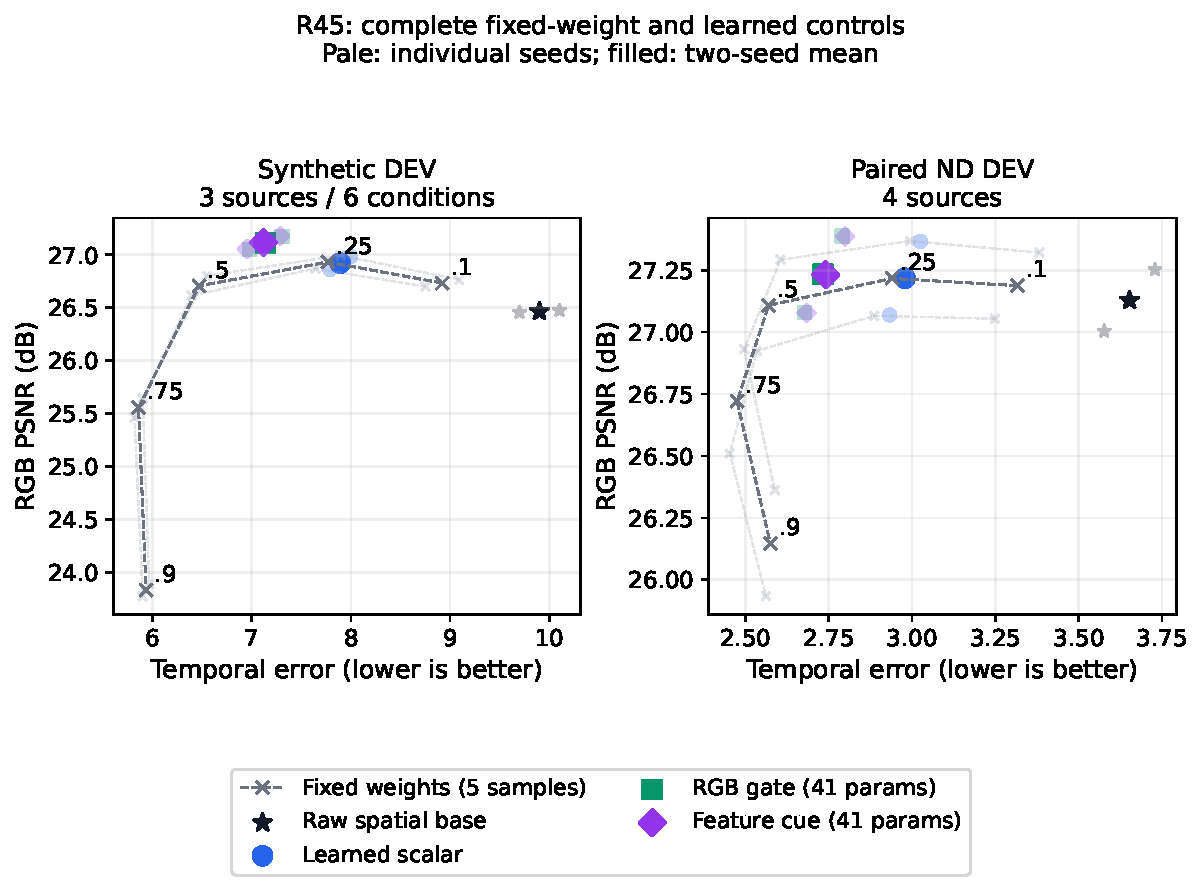
\includegraphics[width=\linewidth]{frontier.pdf}
\caption{Complete R45 fixed-weight sample and learned controls. Pale traces
and points retain both seeds. The RGB and internal-cue gates nearly overlap;
their generic trade-off cannot be credited to an independent internal-cue
mechanism. These are development results, not latency or final-test points.}
\label{fig:r45}
\end{figure}
